\documentclass[11pt]{article}
\addtolength{\oddsidemargin}{-1.cm}
\addtolength{\textwidth}{2cm}
\addtolength{\topmargin}{-2cm}
\addtolength{\textheight}{3.5cm}
\newcommand\tab[1][1cm]{\hspace*{#1}}
\usepackage[pdftex]{graphicx}
\usepackage{pdflscape}
\usepackage[T1]{fontenc}
\usepackage{hyperref}
\usepackage{float}
\usepackage{cite}
\hypersetup{
	colorlinks=true,
	linkcolor=black,
	filecolor=magenta,
	urlcolor=cyan,
}

% define the title
\author{Panda Inc}
\title{Architectural Design Document}
\begin{document}
\begin{titlepage}

	\begin{center}
		% Upper part of the page
        
\includegraphics[width=0.7\linewidth]{images/panda.jpg}\\[1cm]
		\textsc{\LARGE Momentum - Multipy Active Dayz App}\\[0.3cm]
		% Title
		\rule{\linewidth}{0.5mm} \\[1cm]
		{ \huge \bfseries Architectural Design Document}\\[0.5cm]
		\rule{\linewidth}{0.5mm} \\[1cm]


		\begin{minipage}{0.4\textwidth}
			\begin{flushleft} \large
				\emph{} \\
				Quinton {Swanepoel}
			\end{flushleft}
		\end{minipage}
		\begin{minipage}{0.4\textwidth}
			\begin{flushright} \large
				\emph{} \\
				15245510
			\end{flushright}
		\end{minipage}

		\begin{minipage}{0.4\textwidth}
			\begin{flushleft} \large
            	\emph{} \\
				Azhar {Patel}
			\end{flushleft}
		\end{minipage}
		\begin{minipage}{0.4\textwidth}
			\begin{flushright} \large
				\emph{} \\
				15052592
			\end{flushright}
		\end{minipage}

		\begin{minipage}{0.4\textwidth}
			\begin{flushleft} \large
				\emph{} \\
				Tshepo Macebo {Malesela}
			\end{flushleft}
		\end{minipage}
		\begin{minipage}{0.4\textwidth}
			\begin{flushright} \large
				\emph{} \\
				14211582
			\end{flushright}
		\end{minipage}

        \begin{minipage}{0.4\textwidth}
			\begin{flushleft} \large
				\emph{} \\
				Keaton {Pennels}
			\end{flushleft}
		\end{minipage}
		\begin{minipage}{0.4\textwidth}
			\begin{flushright} \large
				\emph{} \\
				14373018
			\end{flushright}
		\end{minipage}

		\rule{\linewidth}{0.5mm} \\[1cm]
		\textsc{\Large Stakeholders}\\[1cm]

		\begin{minipage}{0.4\textwidth}
			\begin{flushleft} \large
				\emph{} \\
				MMI Holdings:
			\end{flushleft}
		\end{minipage}
		\begin{minipage}{0.4\textwidth}
			\begin{flushright} \large
				\emph{} \\
				Phillip Kruger
			\end{flushright}
		\end{minipage}


	\end{center}
\end{titlepage}

\newpage
\paragraph{Abstract}\mbox{}\\
This document serves to describe the architecture used for the ActiveDayz application which is developed for Momentum (Multiply) as part of the Software Engineering Project (COS 301) at the University of Pretoria.\newline
The document complies with the Architectural Design Document Software Engineering Standard, as set by the European Space Agency.



\newpage
\tableofcontents

\newpage

\section{Introduction}
\subsection{Purpose}
Active Dayz is part of Momentum's Multiply wellness and rewards programme. The Active Dayz programme tracks a user's steps taken and calories burned in order to provide users with relevant rewards. The programme currently only works with certain devices. An application is required that can log events such as marathons and other fitness events that users may attend, monitor users gym time, and track users steps taken and calories burned.

\subsection{Scope}
Active Dayz is aimed at providing momentum customers  with a quick way to get rewards/active days by making use of location based services to track when a user goes to gym and how long they stay for.
\newline
\newline
The proposed system is to be integrated with a non-existing admin web interface. It should allow the integration of various services of which location based monitoring is the main objective. Other tools may include monitoring of steps take, calories burned and events attended.

\subsection{Definitions and Abbreviations}
\subsubsection{Definitions}
\subsubsection{Abbreviations}

\subsection{References}
\subsection{Overview}

\section{Architectural Design}
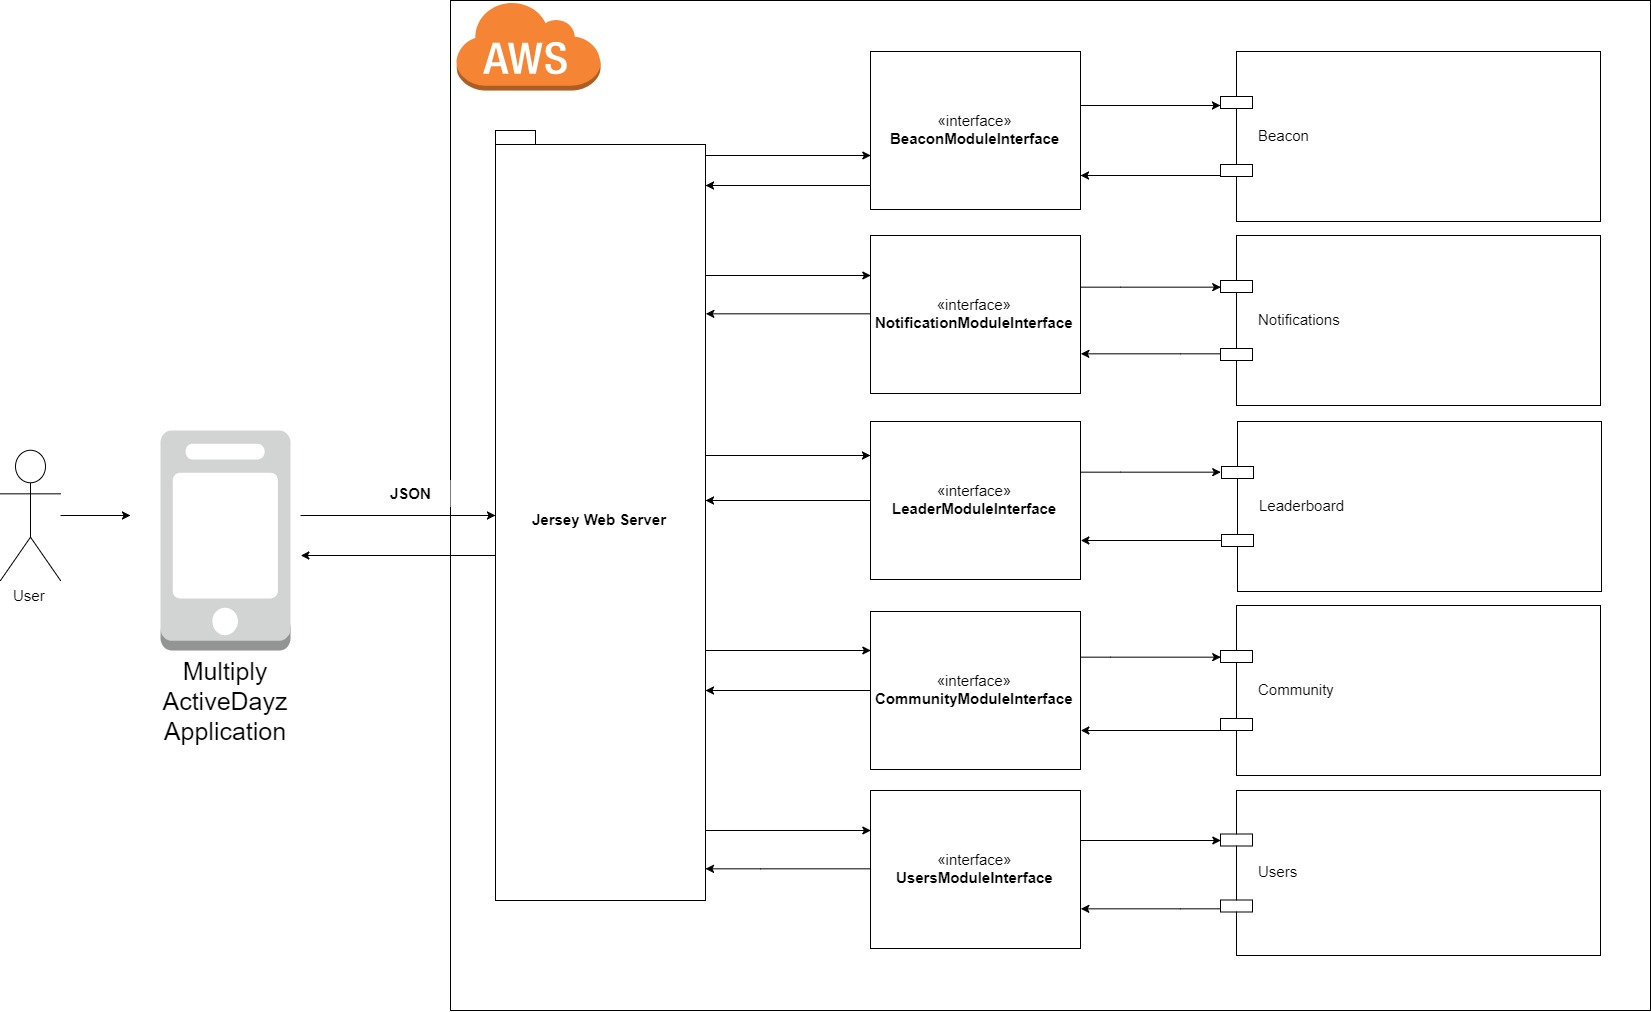
\includegraphics[width=0.7\linewidth]{images/Integration.jpg}\\[1cm]
\subsection{Architectural Patterns of ActiveDayz}
\begin{itemize}
\item Service oriented architecture patterns (Micro services)
\item Layered architecture patterns
\item Event-Driven patterns
\end{itemize}
The first two design patterns were chosen such that the modules within our application would have the as few as possible and also so that we could ensure we achieve low coupling. The event driven pattern will aid in the connecting and ranging of the event driven beacons

\subsection{Quality Requirements/Non functional Requirements}
\begin{itemize}
\item Availability
\item Security
\item Reliability
\item Maintainability
\item Accessibility
\end{itemize}
The above list is the most integral quality requirements for our application and although it is not exhaustive, it encompasses what both our team and the client thought would be necessary for a seamless experience with the application

\subsection{Design Requirements}
\begin{itemize}
\item Our goal is to design a highly modular system which has minimal dependency between the modules
\item The system is required to be designed such that if a module needs to be updated/modified or if a module needs to be added or removed. that this can be done with minimal effort
\end{itemize}



Design Requirement
The system is to be a modular system which allows for
● only a subset of modules to be deployed -- minimally the system will require
the core modules to be deployed.
● further modules, of which the navigation module is the most desirable, to be
added at a later stage.
To this end the system should be implemented with
● minimal dependencies between modules,
● no dependencies of core modules on any add-on modules,
● as far as possible making use of dependency injection.

\section{Component Descriptions}
\subsection{Beacon Module}
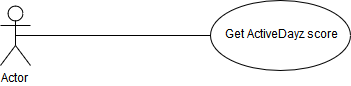
\includegraphics[width=0.7\linewidth]{images/Beacon.png}\\[1cm]
\subsection{Notification Module}
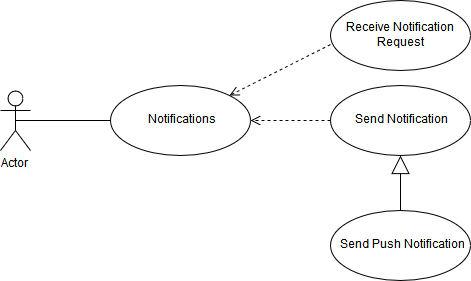
\includegraphics[width=0.7\linewidth]{images/Notification.png}\\[1cm]
\subsection{Leader Module}
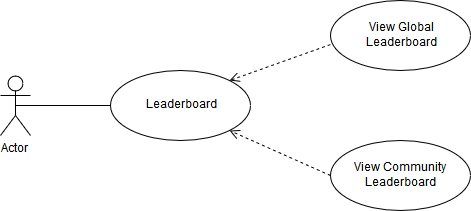
\includegraphics[width=0.7\linewidth]{images/Leaderboard.png}\\[1cm]
\subsection{Community Module}
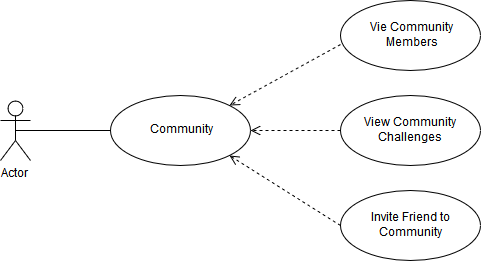
\includegraphics[width=0.7\linewidth]{images/Community1.png}\\[1cm]
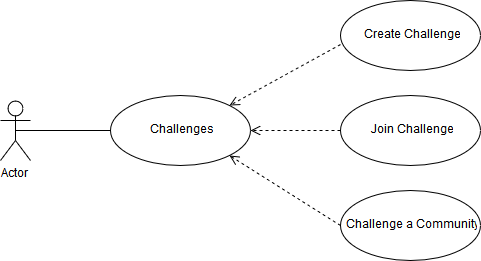
\includegraphics[width=0.7\linewidth]{images/Community2.png}\\[1cm]
\subsection{Users Module}
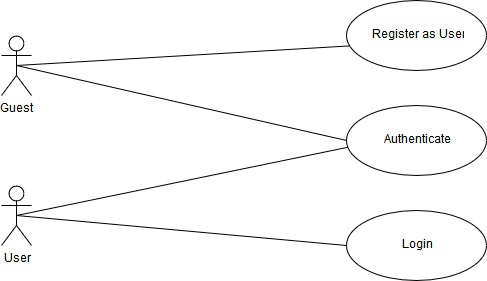
\includegraphics[width=0.7\linewidth]{images/UserManagement.png}\\[1cm]
\subsection{Social Module}
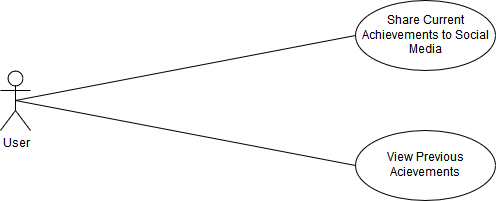
\includegraphics[width=0.7\linewidth]{images/Social.png}\\[1cm]

\section{Feasibility and Resource Estimates}

\section{Technologies Used}
\subsection{Server}
JavaEE eclipse oxygen\\
Jersey restful web service\\
Tomcat App server\\
Amazon aws\\
JSON communication to ensure low coupling\\
Maven build automation\\
\subsection{Web develpement}
polymer\\
node bower and polymer\\
webcomponents\\
js\\
mysql db\\
beacons estimotes\\
docker\\
wildfly\\

\end{document}
